\documentclass{ctexart}
\usepackage{lmodern}
\usepackage{geometry}
\usepackage{fontspec}
\usepackage{amsmath}
\usepackage{amssymb}
\usepackage{mathrsfs}
\usepackage{float}
\usepackage{graphicx}
\usepackage{enumitem}
\usepackage{breqn}
% 页面设置
\geometry{a4paper,scale=0.8,centering}
\pagestyle{plain}

% 项目编号设置
\renewcommand{\theenumii}{\arabic{enumii}}

% 自定义数学命令,这里采用的是教材的定义
\newcommand{\LHS}{\mathrm{LHS}}
\newcommand{\RHS}{\mathrm{RHS}}
\newcommand{\Z}{\mathbb{Z}}
\newcommand{\N}{\mathbb{N}}
\newcommand{\R}{\mathbb{R}}
\newcommand{\Q}{\mathbb{Q}}
\newcommand{\C}{\mathbb{C}}
\newcommand{\E}{\mathbb{E}}
\renewcommand{\O}{\mathcal{O}}
\newcommand{\id}{\mathrm{id}}
\DeclareMathOperator*{\Span}{Span}
\DeclareMathOperator*{\im}{Im}
\DeclareMathOperator*{\rank}{rank}
\DeclareMathOperator*{\card}{card}
\DeclareMathOperator*{\grad}{grad}
\DeclareMathOperator*{\argmax}{argmax}
\DeclareMathOperator*{\epi}{epi}
\DeclareMathOperator*{\maximize}{maximize}
\DeclareMathOperator*{\minimize}{minimize}
\renewcommand{\d}{\mathrm{d}}
\newcommand{\Pow}{\mathcal{P}}
\newcommand{\cov}{\mathsf{Cov}}
\newcommand{\var}{\mathsf{Var}}
\newcommand{\Nor}{\mathcal{N}}
\newcommand{\Poisson}{\mathsf{Poisson}}
\newcommand{\U}{\mathcal{U}}
\renewcommand{\t}{\mathsf{T}}
\newcommand{\T}{\top}
\newcommand{\F}{\bot}
\newcommand{\norm}[1]{\left\|#1\right\|}
\newcommand{\inner}[2]{\left\langle{#1},{#2}\right\rangle}
\newcommand{\e}{\mathrm{e}}
\newcommand{\const}{\mathrm{const}}
\newcommand{\scB}{\mathscr{B}}
\newcommand{\scF}{\mathscr{F}}
\newcommand{\G}{\mathscr{G}}
\newcommand{\Exp}{\mathsf{Exp}}
\newcommand{\DExp}{\mathsf{DExp}}
\newcommand{\Lap}{\mathsf{Lap}}
\newcommand{\calP}{\mathcal P}
\newcommand{\calS}{\mathcal S}
\newcommand{\calF}{\mathcal F}
\newcommand{\calM}{\mathcal M}
\newcommand{\KL}{\mathrm{KL}}
\newcommand{\ReLU}{\mathsf{ReLU}}
\newcommand{\val}{\mathsf{val}}

% 公式换页,1-4分别对应不允许、可能、鼓励、强制换页
\allowdisplaybreaks[3]

% 文档信息
\title{\bfseries 主题一作业}
\author{李二 2300017000}

%% 编译请使用 XeLaTeX
%% 请使用 TeX Live 2024 及以上版本编译

\begin{document}
\maketitle

\section{第一章作业}


%% 请注意,每一个section一个enumerate环境,不要使用多个enumerate环境,否则会导致编号混乱
\begin{enumerate}[wide, labelindent=0pt]
\item[2.] 子问题模板:
\begin{enumerate}
\item 子问题1的回答
\item 子问题2的回答
\end{enumerate}

\item[extra.] 额外问题模板:
其他额外问题

\item[5.] 分类讨论模版:
\begin{itemize}
    \item 情形1:情形1的讨论
    \item 情形2:情形2的讨论
    \begin{itemize}
        \item 情形2.1:情形2.1的讨论
        \item 情形2.2:情形2.2的讨论
        \begin{itemize}
            \item 情形2.2.1:情形2.2.1的讨论
        \end{itemize}
    \end{itemize}
\end{itemize}

\item[6.] 图片模版
\begin{figure}[ht]
    \centering
    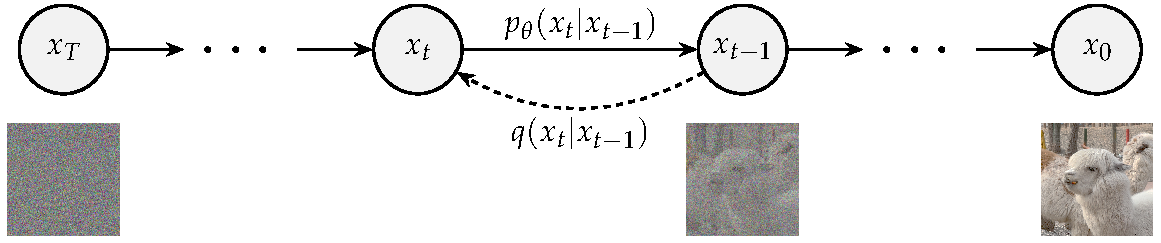
\includegraphics[width=0.7\textwidth]{example-image-a.pdf}
    \caption{图片说明}\label{fig:example}
\end{figure}
引用图片:图 \ref{fig:example}. 

支持多种格式,如PDF、PNG、JPG、EPS、SVG等,推荐使用PDF格式

\item[7.] 表格模版
% 定制表格比较复杂,可以询问 LLM 或者使用在线工具生成
\begin{table}[H]
    \centering
    \begin{tabular}{|c|c|}
        \hline
        1 & 2 \\
        \hline
        3 & 4 \\
        \hline
    \end{tabular}
    \caption{表格说明}\label{tab:example}
\end{table}
引用表格:表 \ref{tab:example}. 

\item[8.] 换行示例

这是第一段

这是第二段

\item[10.] 公式示例

不带编号的公式:

行内公式:$\int_{-\infty}^{+\infty} \exp\left( -\frac{x^2}{2} \right) \d x = \sqrt{2\pi}$

行间公式:
\[
    \int_{-\infty}^{+\infty} \exp\left( -\frac{x^2}{2} \right) \d x = \sqrt{2\pi}
\]

不带编号的多行公式:
\begin{align*}
    \int_{-\infty}^{+\infty} \exp\left( -\frac{x^2}{2} \right) \d x
    &= \sqrt{2\pi} \\
    &= \sqrt{2\pi}
\end{align*}

带编号的公式:
\begin{equation}
    \begin{aligned}
        \frac{1}{2} \left( \frac{1}{\sqrt{2\pi}} \right)^2 \int_{-\infty}^{+\infty} \exp\left( -\frac{x^2}{2} \right) \d x
        &= \frac{1}{2} \left( \frac{1}{\sqrt{2\pi}} \right)^2 \sqrt{2\pi} \\
        &= \frac{1}{4\pi}
    \end{aligned}\label{eq:example-1}
\end{equation}
引用公式:式 \eqref{eq:example-1}. 

多行带编号的公式
\begin{align}
    \frac{1}{2} \left( \frac{1}{\sqrt{2\pi}} \right)^2 \int_{-\infty}^{+\infty} \exp\left( -\frac{x^2}{2} \right) \d x
    &= \frac{1}{2} \left( \frac{1}{\sqrt{2\pi}} \right)^2 \sqrt{2\pi} \label{eq:example-2} \\
        &= \frac{1}{4\pi} \label{eq:example-3}
\end{align}
引用公式:式 \eqref{eq:example-2} 和 \eqref{eq:example-3}. 

\item[11.] 算法请使用itemize环境,不要使用algorithm2e等包,示例:

\begin{itemize}
    \item 对$t=1,2,\ldots$循环执行以下步骤:
    \begin{itemize}
        \item 从分布$P_t$中采样得到样本$x_t$;
        \item 计算梯度$g_t=\nabla f(x_t)$;
        \item 更新参数$x_{t+1}=x_t-\eta_t g_t$. 
    \end{itemize}
\end{itemize}

\item[12.] 流程图请使用tikz包,这个学习曲线比较陡峭,可以询问 LLM 或者查阅文档. 
\end{enumerate}

\section{第二章作业}

\begin{enumerate}[wide, labelindent=0pt]
\item[1.] 其他问题……
\end{enumerate}

\end{document}